
\chapter{Proyecto 2}
\ \\ El proyecto de Pysudoku fue desarrollado en Python.\ \\



\begin{figure}[htbp]
\begin{center}
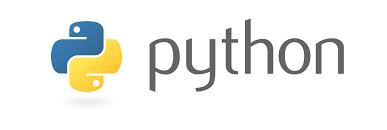
\includegraphics[width=.70\textwidth]{./imagenes/python.jpg}
\caption{qt}
\label{qt}
\end{center}
\end{figure}



El objetivo del segundo Proyecto del Curso de Lenguajes de Programaci\'on fue cambiar de lenguaje nuestro sudoku en QT a Python, en Python que se encontro cambio en la sintaxis instrucciones, un lenguaje mas estructurado por identaciones y una particularidad en el uso de variables se continu\'o trabajando junto a Git como herramienta de versionamiento y el uso de doxygen como herramienta de documentaci\'on.



\ \\
\newpage

\section{Requerimientos del Proyecto PySudoku:}
\ \\ 

Implementar una aplicaci\'on de Sudoku en Python, en la cual podamos validar si la resoluci\'on de un tablero es v\'alida o no es v\'alida.

\ \\ 

Nuestra aplicaci\'on debe generar tableros de sudoku con distintas dificultades.

\ \\ 

Nuestra aplicaci\'on debe mostrarnos ayuda durante la resoluci\'on del tablero mostr\'andonos, cuando un n\'umero ingresado es incorrecto si ya existe en la misma fila, columna o cuadrante

\ \\ 

Nuestra aplicaci\'on debe ofrecernos la opci\'on de mostrar pistas, la cual nos indicar\'a si los numeros ingresados son correctos o incorrectos validando el tablero.

\ \\ 

Nuestra aplicaci\'on nos permitir\'a llevar un registro de los mejores puntajes obtenidos al resolver el tablero en sus diferentes dificultades.

\ \\


\begin{figure}[htbp]
\begin{center}
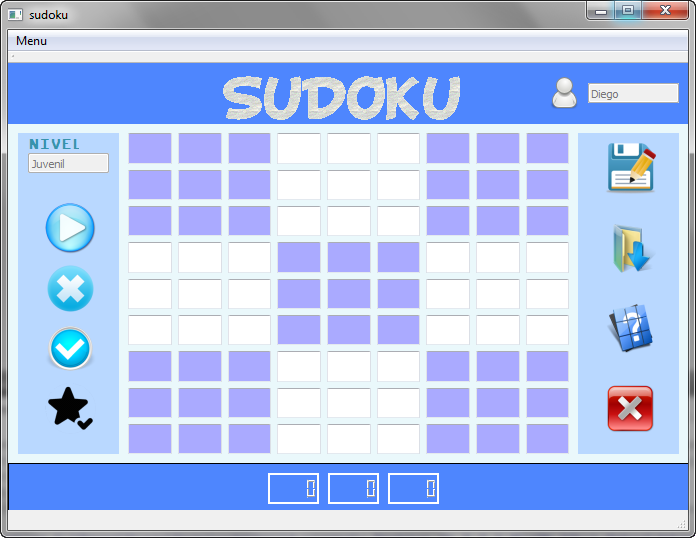
\includegraphics[width=.60\textwidth]{./imagenes/Sudoku.png}
\caption{Tablero Sudoku}
\label{Tablero Sudoku}
\end{center}
\end{figure}


\newpage
\section{Herramientas Utilizadas en el Desarrollo del Proyecto:}

\begin{figure}[htbp]
\begin{center}
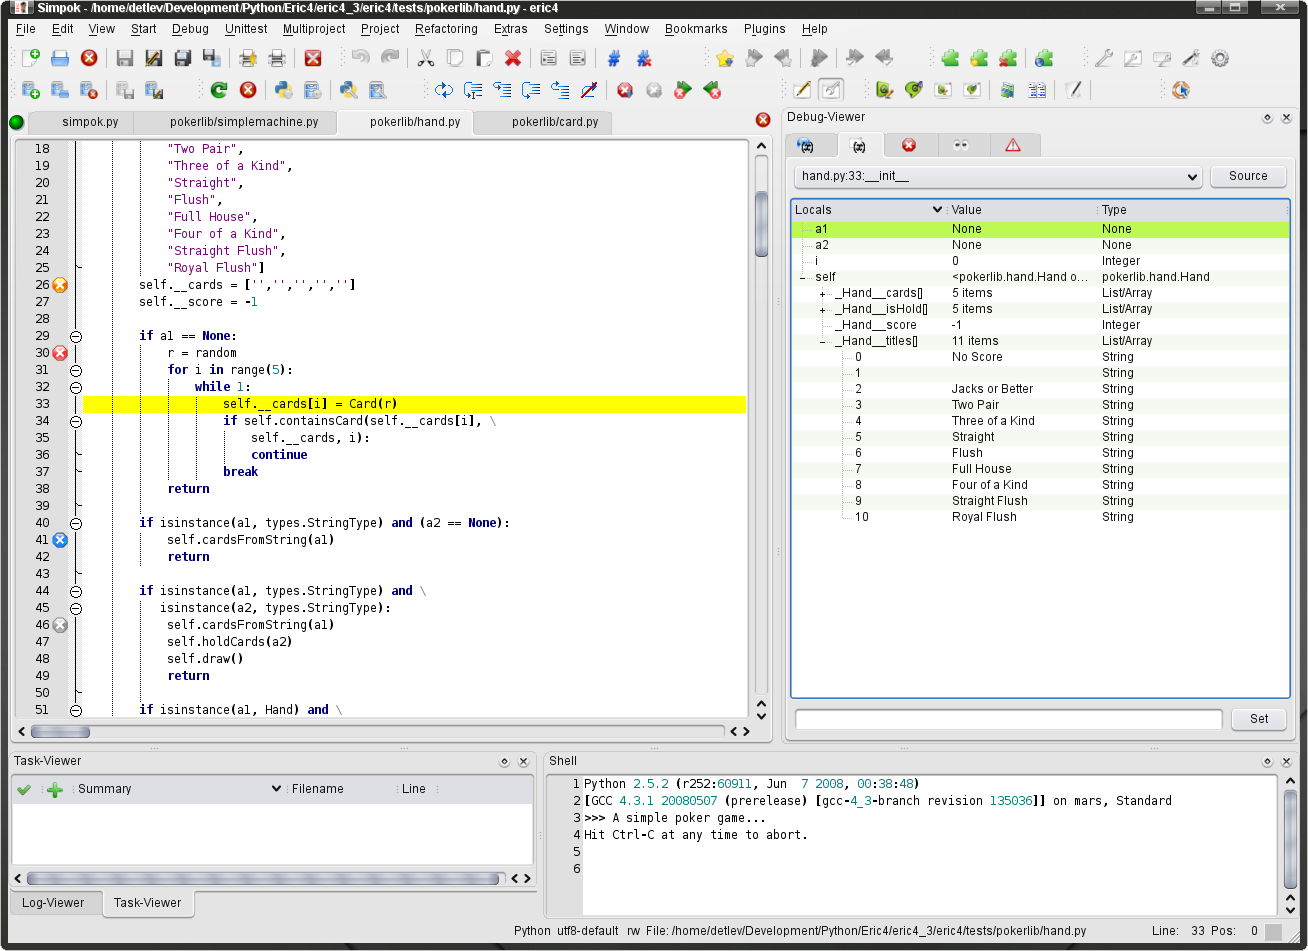
\includegraphics[width=.70\textwidth]{./imagenes/ide_python.png}
\caption{Python}
\label{Python}
\end{center}
\end{figure}

\ \\ 
Python es un lenguaje de programaci\'on interpretado cuya filosof\'\i{}a hace hincapi\'e en una sintaxis muy limpia y que favorezca un c\'odigo legible.
Se trata de un lenguaje de programaci\'on multiparadigma, ya que soporta orientaci\'on a objetos, programaci\'on imperativa y, en menor medida, programaci\'on funcional. Es un lenguaje interpretado, usa tipado din\'amico y es multiplataforma.
Es administrado por la Python Software Foundation. Posee una licencia de c\'odigo abierto, denominada Python Software Foundation License, que es compatible con la Licencia p\'ublica general de GNU a partir de la versi�n 2.1.1, e incompatible en ciertas versiones anteriores.
\ \\


\newpage
\section{GitHub:}
\begin{figure}[htbp]
\begin{center}
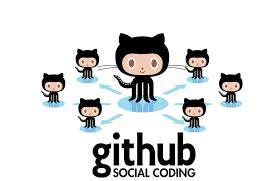
\includegraphics[width=.70\textwidth]{./imagenes/github_logo.jpg}
\caption{git}
\label{git}
\end{center}
\end{figure}

\ \\ 
GitHub es una forja para alojar proyectos utilizando el sistema de control de versiones Git. Utiliza el framework Ruby on Rails por GitHub, Inc. (anteriormente conocida como Logical Awesome).
Desde enero de 2010, GitHub opera bajo el nombre de GitHub, Inc.
El c\'odigo se almacena de forma publica, aunque tambi�n se puede hacer de forma privada, creando una cuenta de pago.
\ \\


\newpage
\section{Doxygen:}
\begin{figure}[htbp]
\begin{center}
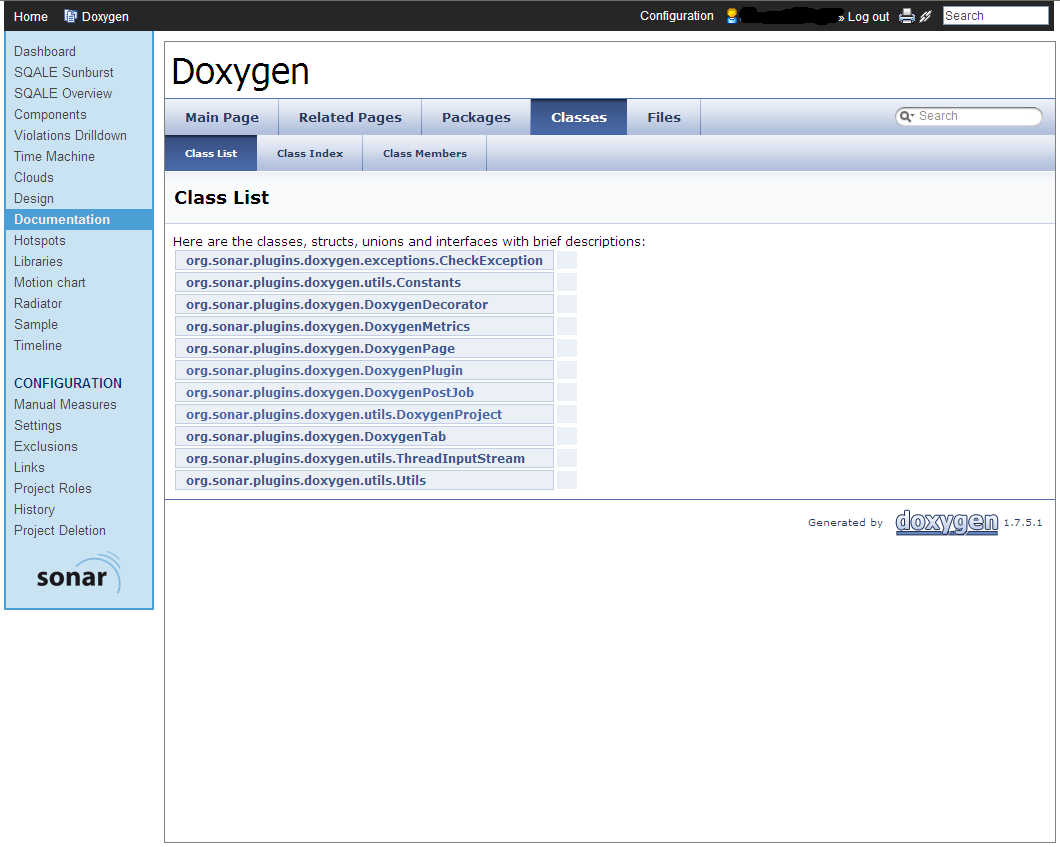
\includegraphics[width=.70\textwidth]{./imagenes/doxygen.png}
\caption{doxygen}
\label{doxygen}
\end{center}
\end{figure}
\ \\ 
Doxygen es un generador de documentaci\'on para C++, C, Java, Objective-C, Python, IDL (versiones Corba y Microsoft), VHDL y en cierta medida para PHP y D. Dado que es f\'acilmente adaptable, funciona en la mayor\'\i{}a de sistemas Unix as� como en Windows y Mac OS X. La mayor parte del c\'odigo de Doxygen esta escrita por Dimitri van Heesch.
Doxygen es un acr\'onimo de dox(document) gen(generator), generador de documentaci\'on para codigo fuente.
Varios proyectos como KDE usan Doxygen para generar la documentacion de su API. KDevelop incluye soporte para Doxygen.
\ \\

\newpage
\section{Objetivos:}
\ \\ 
Crear una aplicaci\'on de sudoku en Python.
\ \\ 
Utilizar Python como principal herramienta de desarrollo.
\ \\ 
Encontrar las ventajas que ofrece Python en comparaci\'on a otros lenguajes antes ulitlizados.
\ \\ 
Implementar la aplicaci\'on con la metodolog\'\i{}a Orientada a objetos en Python.
\ \\ 
Utilizar GIT como herramienta de control de versionamiento.
\ \\ 
Utilizar Doxygen para documentacion del c\'odigo.
\ \\

\section{Desarrollo:}
\ \\ 
El desarrollo de este segundo proyecto se realiz\'o entre dos integrantes del grupo, empezando por crear la interfaz de la aplicaci\'on, que se logr\'o hacerlo importando la interfaz utilizada en QT a Python, luego de esto se procedio a implementar la funcionalidad investigando la sintaxis del Lenguaje para el paso de la funcionalidad de QT a Python.

El trabajo fue dividido entre los dos integrantes del grupo,  Carlos Ram\'\{}irez desarrollo parte de la funcionalidad de las pistas, correcci\'on ingame del sudoku de los n\'umeros ingresados en el tablero por medio del evento textChanged y de la opci\'on de dar pista que permit\'\i{}a mostrar al usuario que valor ingresado era correcto y cual no lo era antes de terminar de llenar el tablero, optimizar ciertas partes del c\'odigo como el momento de generar tableros y la documentaci\'on de la aplicaci\'on. 

Jos\'e V\'elez desarrollo el iniciar partida el cual generaba tableros a partir de una plantilla otra de las funcionalidades implementadas fue el cargar y guardar partida, debidamente encriptado con operaciones de desplazamiento y operaciones aritmeticas al c\'odigo ASCII de los valores del tablero de sudoku. Tambi\'en se encargo de implementar los puntajes que se calculaba en base al tiempo tomado en resolver el juego.

\ \\

\newpage
\section{Conclusiones:}
\ \\ 
La experiencia en Python, como herramienta de trabajo fue satisfactoria debido a que se orientaba a objetos tenia similitudes al lenguaje java, el inconveniente fue el poco tiempo para aprender a manejar la herramienta,una de las ventajas encontradas es que Python es un lenguaje de c\'odigo mejor estructurado por su organizaci\'on por identaci\'on, con la particularidad que no se necesita declarar el tipo de variable, entre las ventajas de Python encontramos, su compatibilidad debido a ser un lenguaje interpretado, una de las desventajas podr\'\i{}a ser un poco menos eficiente en cuestion de tiempo de ejecuci\'on ya que al ser un lenguaje interpretado consume mas recursos que un lenguaje compilado.
\ \\ 
\section{Referencias:}
\ \\ 

	http://mundogeek.net/tutorial-python/

\ \\ 

	http://docs.python.org/2/tutorial/
	
\ \\ 

	http://www.python.org/doc/
	
\ \\ 
\newpage